
\subsection{Bibliothèque \texttt{\gls{game_logic}}}
Dans le chapitre \ref{subsection_architecture_generale} nous avions introduit le module conceptuelle \og Rule Book \fg{}, qui génère un ensemble de pairs coup possible et plateau conséquence. Pour ce faire ce module doit pouvoir décider de la légalité d'un coup et de connaître ses conséquences. 

Nous avions également parlé dans le chapitre \ref{section_analyse_environnement} d'un agent \og Arbitre \fg{} maître du jeu qui a besoin d'un ensemble de règles à fin d'initialiser le plateau et d'appliquer ou de refuser les coups respectivement légaux et illégaux.

Il est claire que ces deux objets partagent un même ensemble de functions et de structures, donc une bibliothèque que nous appelerons \texttt{game\_logic}  :

\begin{figure}[H] 
\centering
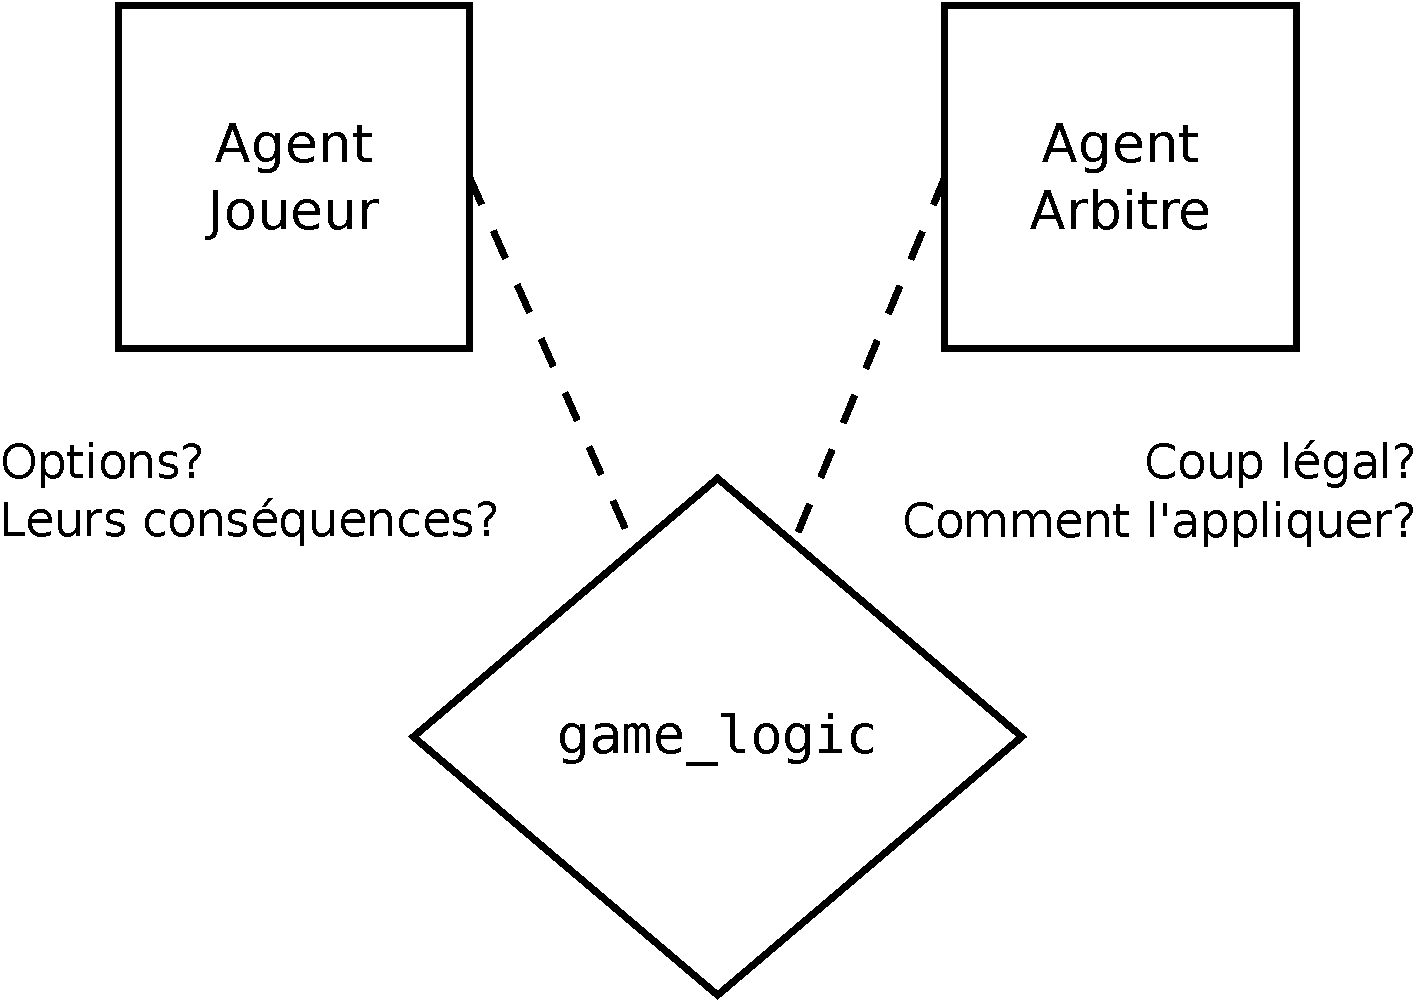
\includegraphics[width=\textwidth]{files/env/game_logic_shared} 
\caption{Partage de la bibliothèque \texttt{game\_logic}} 
\label{game_logic_shared}
\end{figure}

Précisement cette bibliothèque contient trois classes principales :

\begin{itemize}
\item \texttt{BoardMatrix} : Plateau sous forme matricielle avec accesseurs adaptés.
\item \texttt{Rules} : Interface implémenté par chaque jeu. Ses méthodes permettent de connaître :

\begin{itemize}
\item La forme du plateau et sa configuration initiale.
\item Qui joue en premier.
\item Quand la partie est gagné ou perdu et par qui, quand le match est nul.
\item Les coups possibles pour un joueur donnée.
\end{itemize}

\item \texttt{Game} : Associe un \texttt{Rules}, un \texttt{BoardMatrix}, un état et un joueur courant.
\end{itemize}

\begin{figure}[H] 
\centering
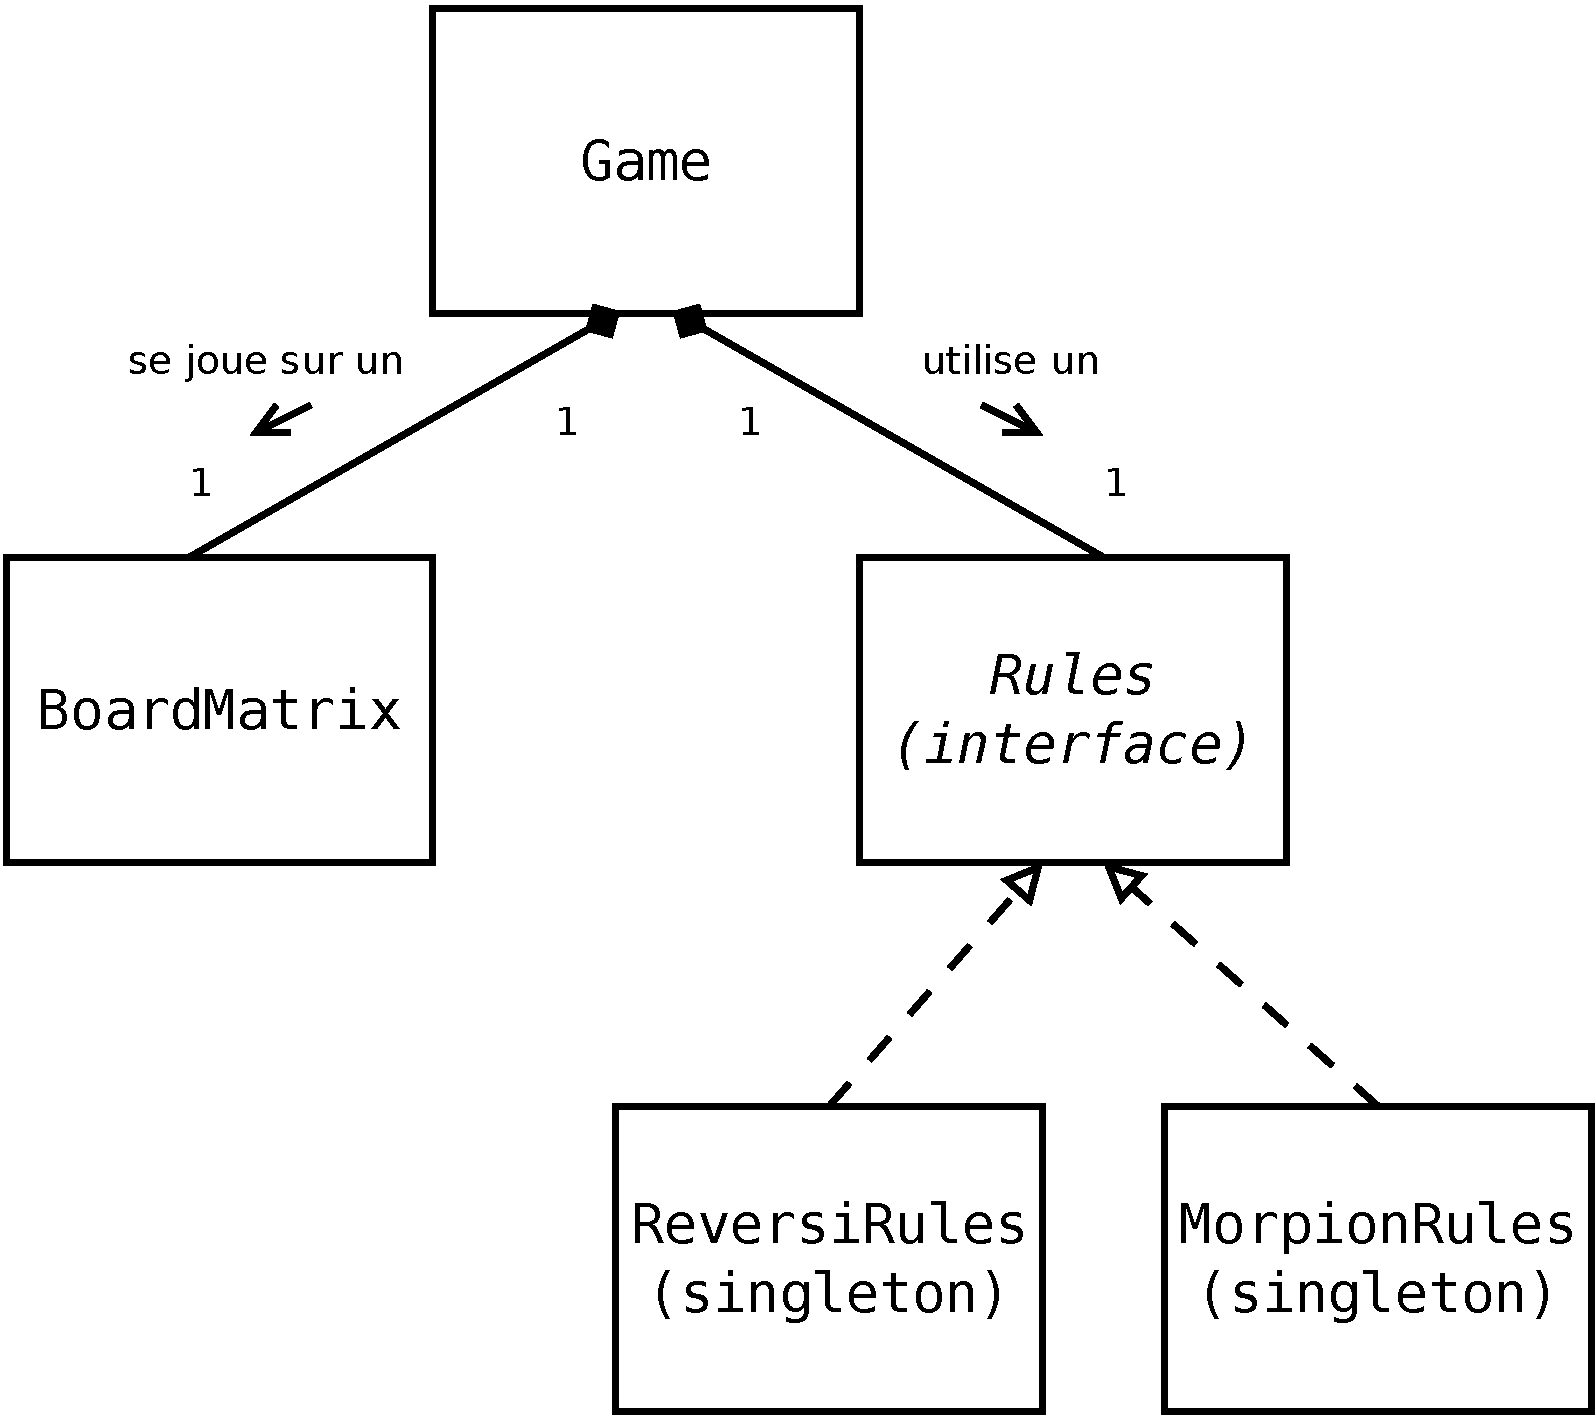
\includegraphics[width=\textwidth]{files/env/game_logic} 
\caption{Classes de la bibliothèque \texttt{game\_logic}} 
\label{game_logic}
\end{figure}